\section{Formalising Credit-Exposures on Decentralised Financial Networks}

A hallmark of decentralised finance is that protocols lock and issue tokens that circulate across multiple platforms.  When a lending protocol such as MakerDAO accepts wrapped ether (WETH) as collateral or a liquidity pool holds stablecoins minted by Circle or Tether, a web of implicit credit links arises: the value of one protocol’s liabilities depends on the solvency and liquidity of another.  Traditional financial network models highlight that interconnectedness can diversify risk but also create channels for contagion; the amplification or dampening of shocks depends on network structure, leverage, and recovery rates \cite{Glasserman2016}.  Early systemic‑risk research used clearing vectors to characterise interbank obligations and showed that fixed‑point algorithms can compute consistent payment outcomes even in the presence of cyclical interdependence \cite{EisenbergNoe2001}.  More recent work demonstrates that as networks become more complete, the stability of the system initially improves but may deteriorate beyond a critical threshold because dense interconnections propagate shocks \cite{Acemoglu2013}.  These insights motivate a rigorous formalisation of credit‑exposure in DeFi networks.

\subsection{Credit Exposure}

Let $X_G(q)$ denote the set of all tokens issued or generated by protocol $q$, and let $X_p(t)$ denote the set of tokens held (or locked) by protocol $p$ at time $t$.  Following \cite{wu2025}, we say that protocol $p$ has {credit exposure} to protocol $q$ at time~$t$ if the tokens it holds include at least one that was issued by $q$:
\begin{equation}
X_p(t)\cap X_G(q)\neq \varnothing.
\label{eq:credit-exposure-definition}
\end{equation}
In other words, $p$ holds a liability of $q$; if the tokens issued by $q$ lose value or become illiquid, then $p$ faces a corresponding loss.  This token‑mediated dependence generalises the notion of counterparty credit risk in traditional finance to decentralised platforms, where exposures arise not from explicit bilateral contracts but from the possession of tokenised claims.  The DeXposure dataset measures the dynamics of these relationships by reconstructing total value locked (TVL) time series for each protocol and tracking how the composition of tokens held by each protocol evolves over time.

%\subsection{Illustrative example}

\begin{figure}[htbp]
    \centering
    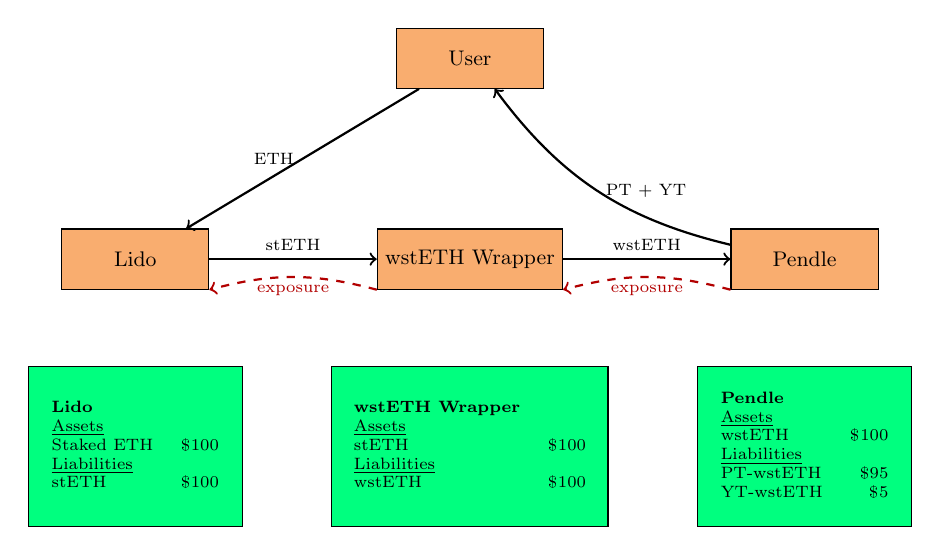
\begin{tikzpicture}[node distance=2.5cm, auto, scale=0.85, transform shape]
        \tikzstyle{entity} = [rectangle, draw, fill=Apricot, minimum width=2.2cm, minimum height=0.9cm, font=\small]
        \tikzstyle{balance} = [rectangle, draw, fill=SpringGreen, minimum width=3.2cm, minimum height=2.4cm, font=\scriptsize]
        \tikzstyle{exposure} = [->, thick, dashed, red!70!black]

        % User at top
        \node[entity] (user) at (0,3) {User};

        % Three protocols in a row
        \node[entity] (lido) at (-5,0) {Lido};
        \node[entity] (wrapper) at (0,0) {wstETH Wrapper};
        \node[entity] (pendle) at (5,0) {Pendle};

        % Balance sheets below each protocol
        \node[balance] (balanceLido) at (-5,-2.8) {
            \begin{tabular}{lr}
                \textbf{Lido} & \\
                \underline{Assets} & \\
                Staked ETH & \$100 \\
                \underline{Liabilities} & \\
                stETH & \$100
            \end{tabular}
        };
        \node[balance] (balanceWrapper) at (0,-2.8) {
            \begin{tabular}{lr}
                \textbf{wstETH Wrapper} & \\
                \underline{Assets} & \\
                stETH & \$100 \\
                \underline{Liabilities} & \\
                wstETH & \$100
            \end{tabular}
        };
        \node[balance] (balancePendle) at (5,-2.8) {
            \begin{tabular}{lr}
                \textbf{Pendle} & \\
                \underline{Assets} & \\
                wstETH & \$100 \\
                \underline{Liabilities} & \\
                PT-wstETH & \$95 \\
                YT-wstETH & \$5
            \end{tabular}
        };

        % Token flows (solid arrows)
        \draw[->, thick] (user) -- node[left, font=\scriptsize] {ETH} (lido);
        \draw[->, thick] (lido) -- node[above, font=\scriptsize] {stETH} (wrapper);
        \draw[->, thick] (wrapper) -- node[above, font=\scriptsize] {wstETH} (pendle);
        \draw[->, thick] (pendle) to[bend left=20] node[right, font=\scriptsize] {PT + YT} (user);

        % Credit exposure arrows (dashed red)
        \draw[exposure] (pendle.south west) to[bend right=15] node[below, font=\scriptsize, text=red!70!black] {exposure} (wrapper.south east);
        \draw[exposure] (wrapper.south west) to[bend right=15] node[below, font=\scriptsize, text=red!70!black] {exposure} (lido.south east);

    \end{tikzpicture}
    \caption{Multi-layer credit exposure in DeFi. A user stakes ETH with Lido, receiving stETH, which is wrapped into wstETH and deposited into Pendle. Each protocol holds the liability of the preceding one, creating a chain of credit exposures from Pendle to Lido.}
    \label{fig:exposure_example}
\end{figure}

\noindent Figure~\ref{fig:exposure_example} illustrates how a single user transaction creates a multi-layer chain of credit exposures in DeFi.  A user deposits ETH into Lido, a liquid staking protocol, and receives stETH, a rebasing token that accrues staking rewards.  The stETH is then wrapped into wstETH, a non-rebasing representation that is more compatible with DeFi protocols.  Finally, wstETH is deposited into Pendle, a yield-tokenisation protocol that splits the asset into a principal token PT-wstETH and a yield token YT-wstETH, allowing users to trade fixed and variable yield separately.

In balance-sheet terms, Lido holds staked ETH with validators and issues stETH as liabilities, the wstETH wrapper holds stETH and issues wstETH, and Pendle holds wstETH and issues the PT and YT pair.  Because each protocol's assets consist of tokens issued by the preceding protocol, a chain of credit exposures emerges: Pendle has exposure to the wstETH wrapper, which in turn has exposure to Lido.  If Lido experienced a slashing event or stETH de-pegged from ETH, the losses would cascade through wstETH and into Pendle, affecting PT and YT holders.  This example demonstrates that DeFi exposures are inherently multi-layered, as liquid staking, wrapping, and yield tokenisation compound into complex dependency structures that the DeXposure dataset aims to capture.

\subsection{Mapping Tokens to Issuing Protocols}

To operationalise \eqref{eq:credit-exposure-definition}, we must determine which protocol issues each token and thus identify the direction of exposure.  Let $\mathcal{P}$ denote the set of all protocols and $\mathcal{C}$ the set of blockchains.  For each token $\sigma$ appearing in protocol $p$, a \textbf{mapping function} $M(\sigma)$ returns the protocol $q$ that issues or manages $\sigma$.  The DeXposure dataset constructs $M$ using a fall‑back procedure:
\begin{enumerate}
  \item \textbf{Metadata lookup:} Tokens are directly matched to issuing protocols using metadata from DefiLlama when available.
  \item \textbf{Manual mapping:} For tokens with high TVL that lack metadata links, researchers manually assign the issuing protocol based on documentation and expert knowledge.
  \item \textbf{Text‑vector similarity:} For remaining tokens, the text descriptions of tokens and protocols are vectorised via the term frequency–inverse document frequency (TF--IDF) representation \cite{Qaiser2018}.  Cosine similarity scores between token and protocol vectors determine the best match, and tokens are mapped to the protocol with the highest similarity score exceeding a threshold $\theta$.
  \item \textbf{Primary market tokens:} If none of the above methods yields a mapping, the token is treated as its own protocol (e.g., WETH).
\end{enumerate}
This mapping ensures that token flows between protocols can be attributed to changes in credit exposure with respect to the correct issuing protocol, even when tokens are bridged across chains or wrapped by multiple platforms.

\subsection{Network Representation and Value Flows}

Credit exposures over a discrete time interval $\tau = t_2 - t_1$ are represented by a weighted directed graph $G_\tau = (P_\tau, E_\tau)$, where $P_\tau$ is the set of active protocols and $E_\tau$ is the set of directed edges.  Each vertex $p\in P_\tau$ is assigned a \textbf{node weight} equal to the value of assets it holds at the end of the interval:
\begin{equation}
w_\tau(p) = \sum_{\sigma\in X_p(t_1)\cap X_p(t_2)} v_{t_2,\sigma},
\label{eq:node-weight}
\end{equation}
where $v_{t_2,\sigma}$ is the USD value of token $\sigma$ at time $t_2$.  Nodes with negligible weight (below a threshold $\theta$) can be pruned for clarity.  To define the \textbf{edge weight} from protocol $p$ to protocol $q$, we first compute the value flow for each token $\sigma$:
\begin{equation}
F^{\sigma}_{p q,\tau} =
\begin{cases}
\max\bigl(0,\, -\Delta S^{\sigma}_{p,\tau}\bigr), & \text{if } \Delta S^{\sigma}_{p,\tau} < 0,\\
\max\bigl(0,\,\Delta S^{\sigma}_{q,\tau}\bigr), & \text{if } \Delta S^{\sigma}_{q,\tau} \ge 0,
\end{cases}
\label{eq:value-flow}
\end{equation}
where $\Delta S^{\sigma}_{p,\tau}=v_{p,t_2}^{\sigma}-v_{p,t_1}^{\sigma}$ is the change in the USD value of token $\sigma$ held by protocol $p$ over the interval.  Equation~\eqref{eq:value-flow} captures the intuition that if $p$ decreases its holdings of $\sigma$ and $q$ increases theirs, then $\sigma$ has flowed from $p$ to $q$; negative flows are reversed so that all flows are non‑negative.  The \textbf{edge weight} $w_\tau(e_{p q})$ is the sum of flows for all tokens that map to the issuing protocol $q$:
\begin{equation}
w_\tau(e_{p q}) = \sum_{\sigma \in X_{p q, \tau}} F^{\sigma}_{p q,\tau},
\label{eq:edge-weight}
\end{equation}
where $X_{p q,\tau}$ denotes the set of tokens with issuing protocol $q$ that move from $p$ to $q$ over $\tau$.  A positive edge weight indicates increasing exposure from $p$ to $q$.  For single‑token protocols, the flow of that token equals the edge weight.

Algorithm~1 in \cite{wu2025} describes a procedure for constructing $G_\tau$ from raw token‑protocol‑chain mappings.  In summary, one aggregates token holdings at the start and end of the interval, computes node weights, discards nodes below a threshold, and then computes edge weights by summing positive flows; negative flows are reversed to ensure all weights are non‑negative.  The resulting time‑indexed sequence of graphs captures the evolving structure of credit dependencies in the DeFi ecosystem.

\subsection{Discussion and links to systemic‑risk theory}

The above formalism bridges decentralised finance with established theories of financial networks.  By modelling credit exposures as weighted directed graphs derived from token flows, it becomes possible to apply systemic‑risk measures, such as centrality metrics, contagion indices, and stress tests, developed for interbank networks to DeFi.  Classical models show that fixed‑point algorithms can compute consistent clearing payments for interbank systems with cyclic obligations \cite{EisenbergNoe2001}, and that network structures can either buffer or amplify shocks depending on leverage and liquidity \cite{Glasserman2016}.  \cite{Acemoglu2013} further demonstrate that more complete networks initially enhance stability by distributing losses across many counterparties, but beyond a critical density the same interconnections propagate shocks and increase systemic fragility.  In the DeFi context, our graph formalisation reveals similar trade‑offs: diversifying collateral across multiple protocols may reduce reliance on any single issuer, yet highly interconnected protocols could become conduits for contagion if a stablecoin or wrapped token suffers a de‑peg or exploit.

This mathematical framework provides the foundation for the downstream tasks tackled by DeXposure‑FM.  Forecasting future node and edge weights, stress‑testing scenarios under shocks to token values, and imputing missing TVL data all rely on accurate representations of credit exposure.  Moreover, the network perspective aligns with macroprudential policy goals: regulators can monitor systemic importance and spillover risks by examining the temporal evolution of $G_\tau$, and researchers can evaluate how proposed protocol designs or regulatory interventions would reshape the exposure network.  As decentralised finance continues to grow and integrate with the broader financial system, rigorous formalisation and measurement of credit exposure will be essential for safeguarding stability and fostering responsible innovation.